% Este documento tem a ver com as partes do LIVRO. 

\input{1-fronte}       % [Frontistício]
%\input{2-creditos}     % [Créditos]
\input{3-rosto}	       % [folha de rosto]
% nothing			is level -3
% \book				is level -2
% \part				is level -1
% \chapter 			is level 0
% \section 			is level 1
% \subsection 		is level 2
% \subsubsection 	is level 3
% \paragraph 		is level 4
% \subparagraph 	is level 5
\setcounter{secnumdepth}{-2}
\setcounter{tocdepth}{0}

% \renewcommand{\contentsname}{Índex} 	% Trocar nome do sumário para 'Índex'
%\ifodd\thepage\relax\else\blankpage\fi 	% Verifica se página é par e coloca página branca
%\tableofcontents*

\pagebreak
\begingroup \footnotesize \parindent0pt \parskip 5pt \thispagestyle{empty} \vspace*{-0.5\textheight}\mbox{} \vfill
\baselineskip=.92\baselineskip
\textbf{O que Eliane Salama cozinha} \lipsum[2]




\endgroup

\pagebreak
{\begingroup\mbox{}\pagestyle{empty}
\pagestyle{empty} 
% \renewcommand{\contentsname}{Índex} 	% Trocar nome do sumário para 'Índex'
%\ifodd\thepage\relax\else\blankpage\fi 	% Verifica se página é par e coloca página branca
\addtocontents{toc}{\protect\thispagestyle{empty}}
\tableofcontents*\clearpage\endgroup}

\openany
% \blankpage
% \part[O que Eliane S. nos conta sobre cozinha]{{\itshape O que\\ \emph{Eliane S.}\\ nos conta sobre cozinha}}
\blankpage

\thispagestyle{empty}
\clearpage
\begin{tikzpicture}[remember picture, overlay]
\node at (3,-7) {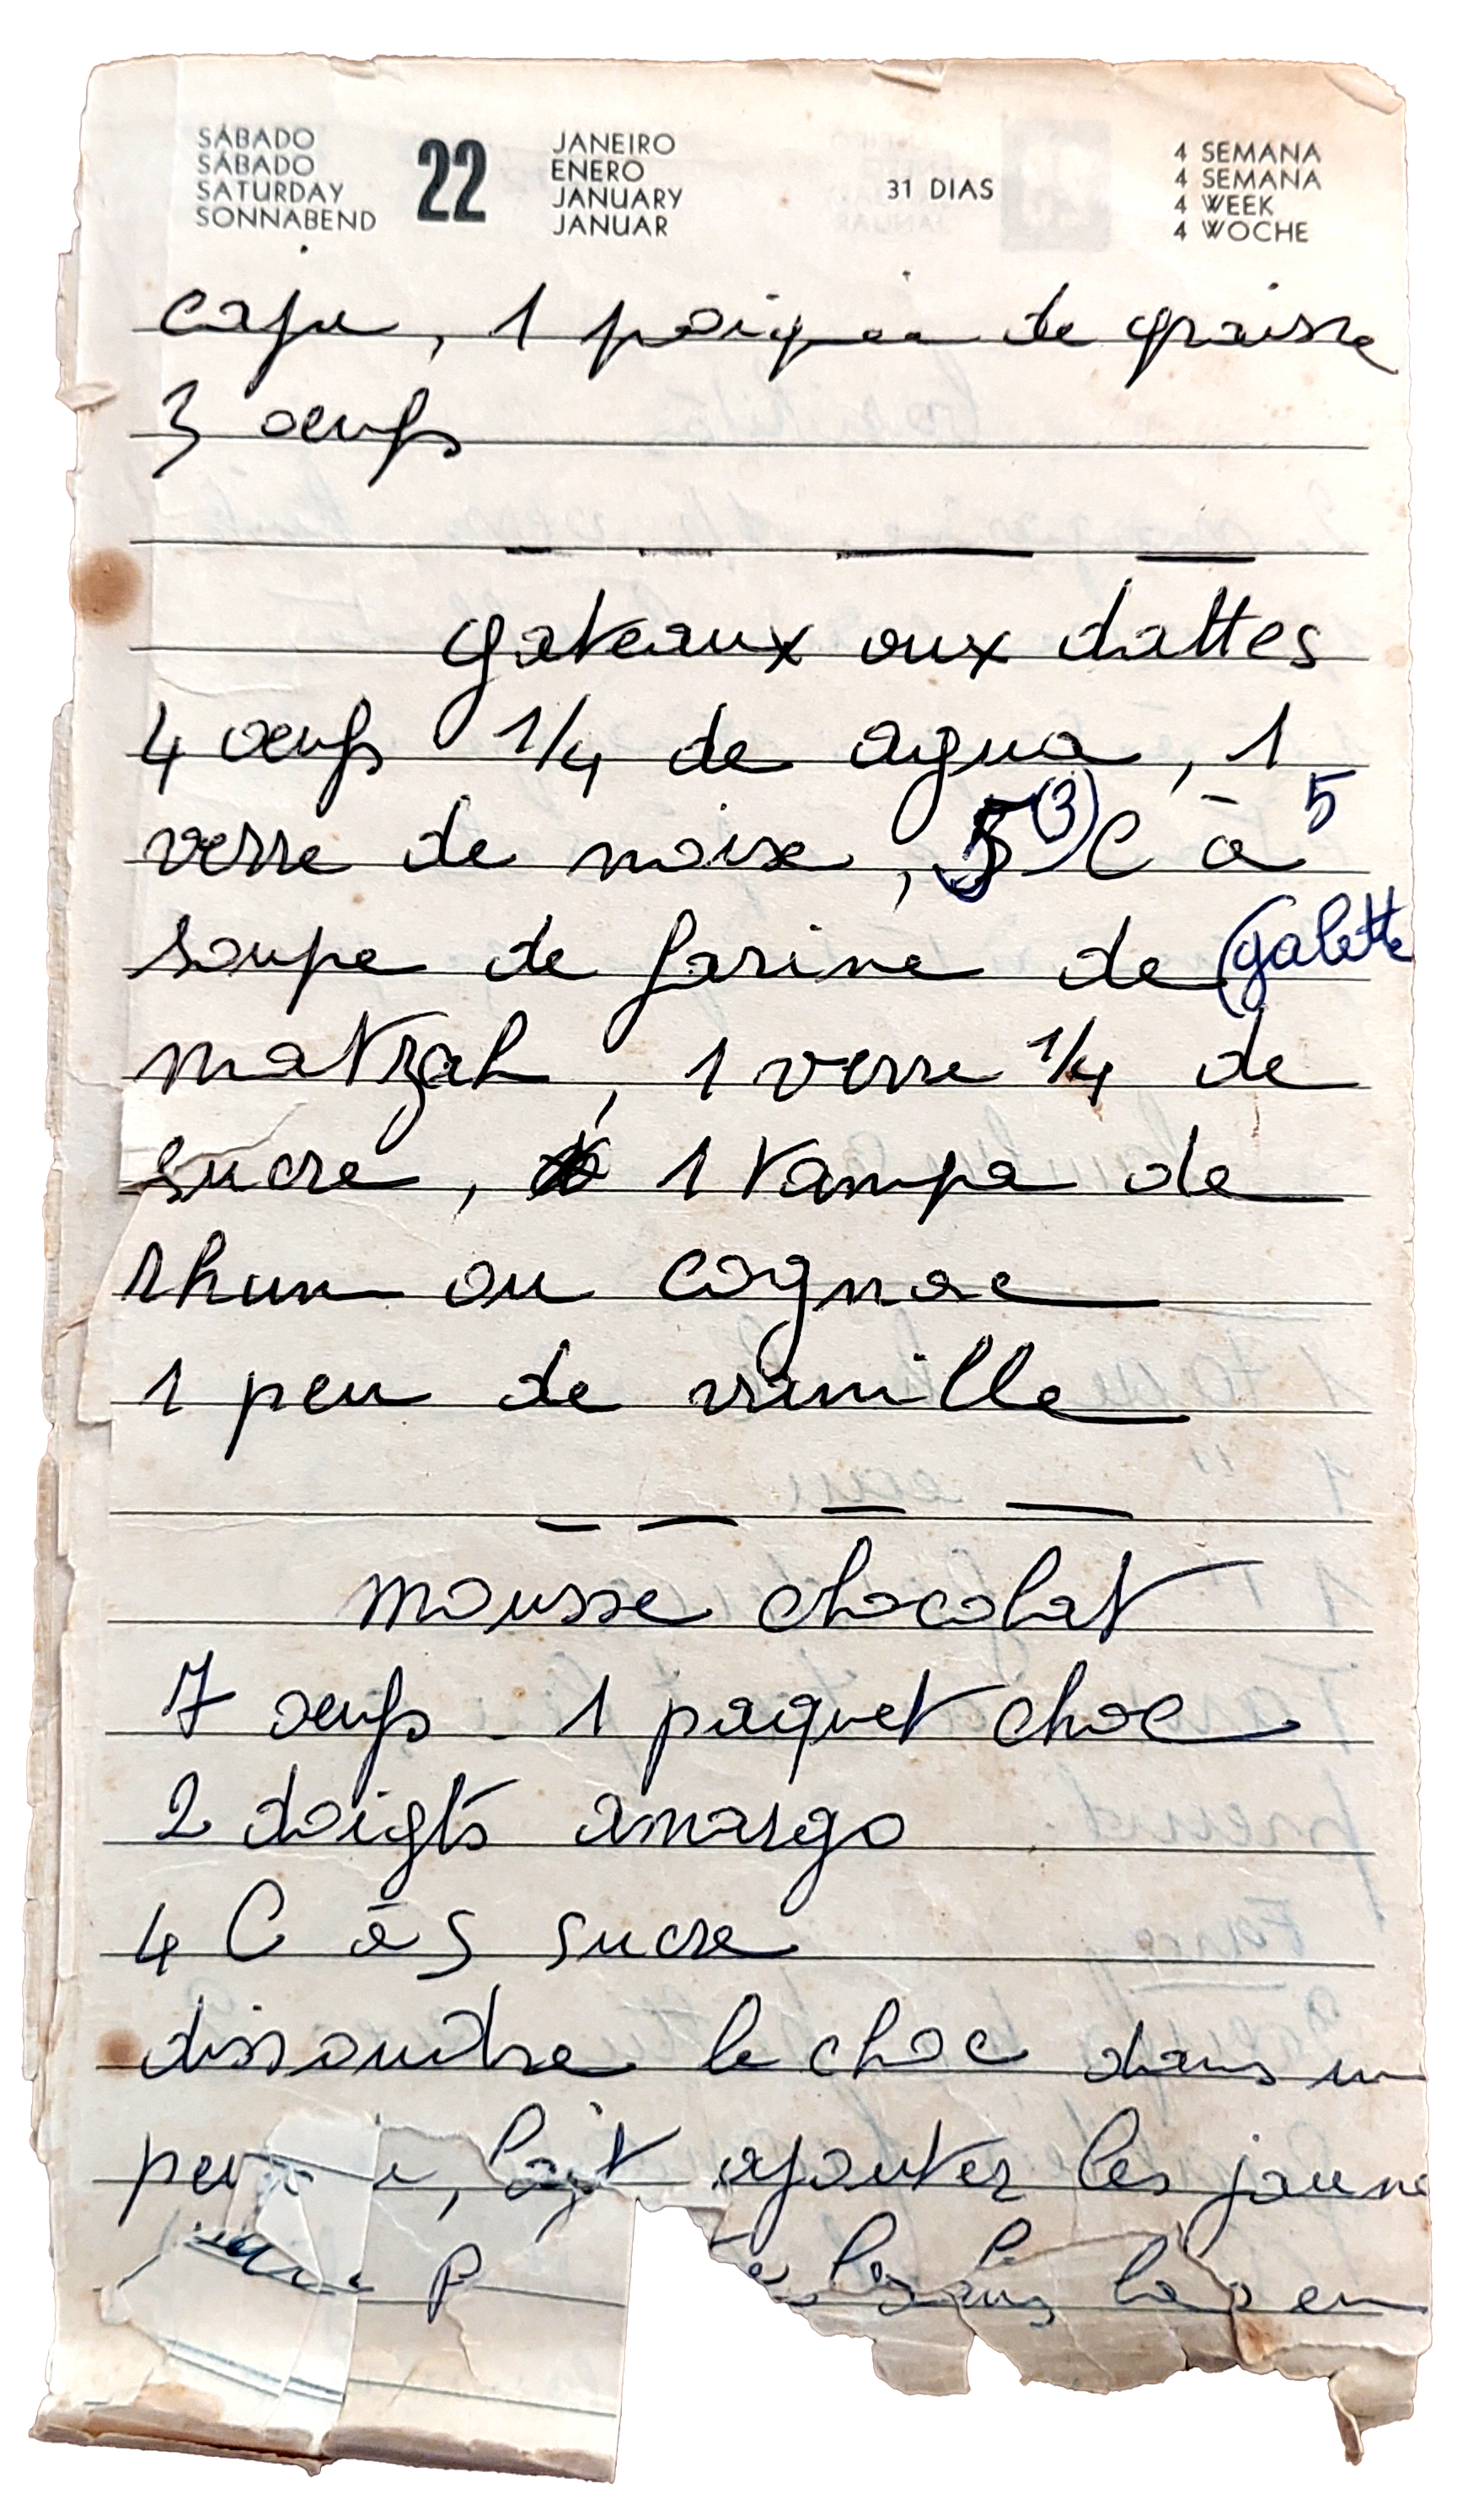
\includegraphics[width=8cm]{./recettes/edités/Gateau aux dattes et Mousse chocolat.jpg}}; 
\end{tikzpicture}\clearpage\thispagestyle{empty}
% \begin{tikzpicture}[remember picture,overlay]
% \fill[black] (-3,3.5) rectangle (14,-21.5);
% \end{tikzpicture}
\clearpage

\chapter*{Gâteau aux dattes}

\section{Ingrédients originaux}

\begin{itemize}
\item 4 œufs
\item 1 verre de noix
\item 5 c à soupe de farine de galette matzá
\item 1/4 verre de sucre
\item 1 tampo de rhum ou cognac
\item un peu de vanille
\end{itemize}

\section{Préparation adaptée}

Battez les œufs avec le sucre jusqu’à obtenir un mélange clair. Ajoutez le cognac et deux cuillères à soupe de vanille en mélangeant bien. Incorporez la farine de matsá, puis ajoutez les noix et les dattes hachées selon votre goût (si elles sont sèches, hydratez-les rapidement dans de l’eau tiède). Mélangez jusqu’à obtenir une pâte homogène, en ajustant la texture avec un peu de liquide si nécessaire ; versez dans un moule beurré et faites cuire au four préchauffé à 180°,\textsc{c} pendant environ 30 à 40 minutes, jusqu’à ce que le gâteau soit doré et ferme.

\chapter{Bolo de tâmaras}

\section{Ingredientes originais}

\begin{itemize}
\item 4 ovos
\item 1 copo de nozes
\item 5 colheres de sopa de farinha de matzá
\item 1/4 de copo de açúcar
\item 1 tampinha de rum ou conhaque
\item Um pouco de baunilha
\end{itemize}

\section{Modo de preparo adaptado}

Bata os ovos com o açúcar até obter uma mistura clara. Adicione o conhaque e duas colheres de sopa de baunilha, misturando bem. Incorpore a farinha de matzá e, em seguida, acrescente as nozes e as tâmaras picadas a gosto (se estiverem secas, hidrate rapidamente em água morna). Misture até obter uma massa homogênea, ajustando a textura com um pequeno pouco de líquido se necessário; despeje em uma forma untada e leve ao forno preaquecido a 180°\,\textsc{c} por cerca de 30 a 40 minutos, até dourar e firmar.
\blankpage

\thispagestyle{empty}
\clearpage
\begin{tikzpicture}[remember picture, overlay]
\node at (3,-7) {\includegraphics[width=8cm]{./recettes/edités/Biscuit vanille et Biscuit à l'anis.jpg}}; 
\end{tikzpicture}\clearpage\thispagestyle{empty}
% \begin{tikzpicture}[remember picture,overlay]
% \fill[black] (-3,3.5) rectangle (14,-21.5);
% \end{tikzpicture}
\clearpage

\chapter*{Biscuits à l’anis}

\section{Ingrédients originaux}

\begin{itemize}
\item 3 œufs
\item 1/2 verre huile
\item 150 gr. de sucre
\item 1 poignée d’anis
\item Farine autant que ça prend
\end{itemize}

\section{Préparation adaptée}

Battez les œufs avec le sucre jusqu’à obtenir un mélange clair et homogène, ajoutez l’huile puis l’anis. Incorporez la farine progressivement jusqu’à obtenir une pâte molle, souple et légèrement collante. Ajoutez la levure chimique (\textsc{b.\,p.}) en comptant environ 1 cuillère à café pour chaque verre de farine utilisé. Formez des petites boules ou des biscuits légèrement aplatis, disposez-les sur une plaque et faites cuire au four préchauffé à 180°\,\textsc{c} pendant 15 à 25 minutes, jusqu’à ce qu’ils soient légèrement dorés.

\chapter{Biscoitos de anis}

\section{Ingredientes originais}

\begin{itemize}
\item 3 ovos
\item 1/2 copo de óleo
\item 150 g de açúcar
\item 1 punhado de anis
\item Farinha quanto baste
\end{itemize}

\section{Modo de preparo adaptado}

Bata os ovos com o açúcar até obter uma mistura clara e homogênea, adicione o óleo e depois o anis. Incorpore a farinha aos poucos até obter uma massa macia, maleável e levemente pegajosa. Adicione o fermento químico calculando cerca de 1 colher de chá para cada copo de farinha utilizado. Modele pequenas bolinhas ou biscoitos levemente achatados, disponha-os em uma assadeira e leve ao forno preaquecido a 180°,\textsc{c} por 15 a 25 minutos, até ficarem levemente dourados.
\blankpage

\thispagestyle{empty}
\clearpage
\begin{tikzpicture}[remember picture, overlay]
\node at (3,-7) {\includegraphics[width=8cm]{./recettes/edités/Tarte suisse de coco (versão 1).jpg}}; 
\end{tikzpicture}\clearpage\thispagestyle{empty}
% \begin{tikzpicture}[remember picture,overlay]
% \fill[black] (-3,3.5) rectangle (14,-21.5);
% \end{tikzpicture}
\clearpage

\chapter*{Tarte suisse de coco}

\section{Ingrédients originaux}

\begin{itemize}
\item 1 verre noix de coco
\item 5 œufs
\item 2 verres farine
\item 2 verres sucre
\item 1 verre lait
\item 1 paquet beurre
\item 1 c. à s. baking
\item Vanille
\end{itemize}

\section{Préparation adaptée}

Travaillez le beurre (150--200 g.) avec 1 verre de sucre ; ajoutez les œufs, puis le lait, la vanille et la noix de coco râpée ; incorporez la farine jusqu’à obtenir une pâte homogène et ajoutez la levure. Faites cuire dans un moule beurré à 180°,\textsc{c} pendant 35--45 min. ; préparez un sirop avec 1 verre de sucre, de l’eau et du citron, portez à ébullition et arrosez le gâteau encore chaud en laissant absorber.

\chapter{Torta suíça de coco}

\section{Ingredientes originais}

\begin{itemize}
\item 1 copo de coco ralado
\item 5 ovos
\item 2 copos de farinha
\item 2 copos de açúcar
\item 1 copo de leite
\item 1 tablete de manteiga
\item 1 colher de sopa de fermento em pó
\item Baunilha
\end{itemize}

\section{Modo de preparo adaptado}

Bata a manteiga (150--200 g.) com 1 copo de açúcar; adicione os ovos, depois o leite, a baunilha e o coco ralado; incorpore a farinha até obter uma massa homogênea e misture o fermento. Asse em forma untada a 180°,\textsc{c} por 35–45 min.; prepare uma calda com 1 copo de açúcar, água e limão, ferva e regue o bolo ainda quente, deixando absorver.
\blankpage

\thispagestyle{empty}
\clearpage
\begin{tikzpicture}[remember picture, overlay]
\node at (3,-7) {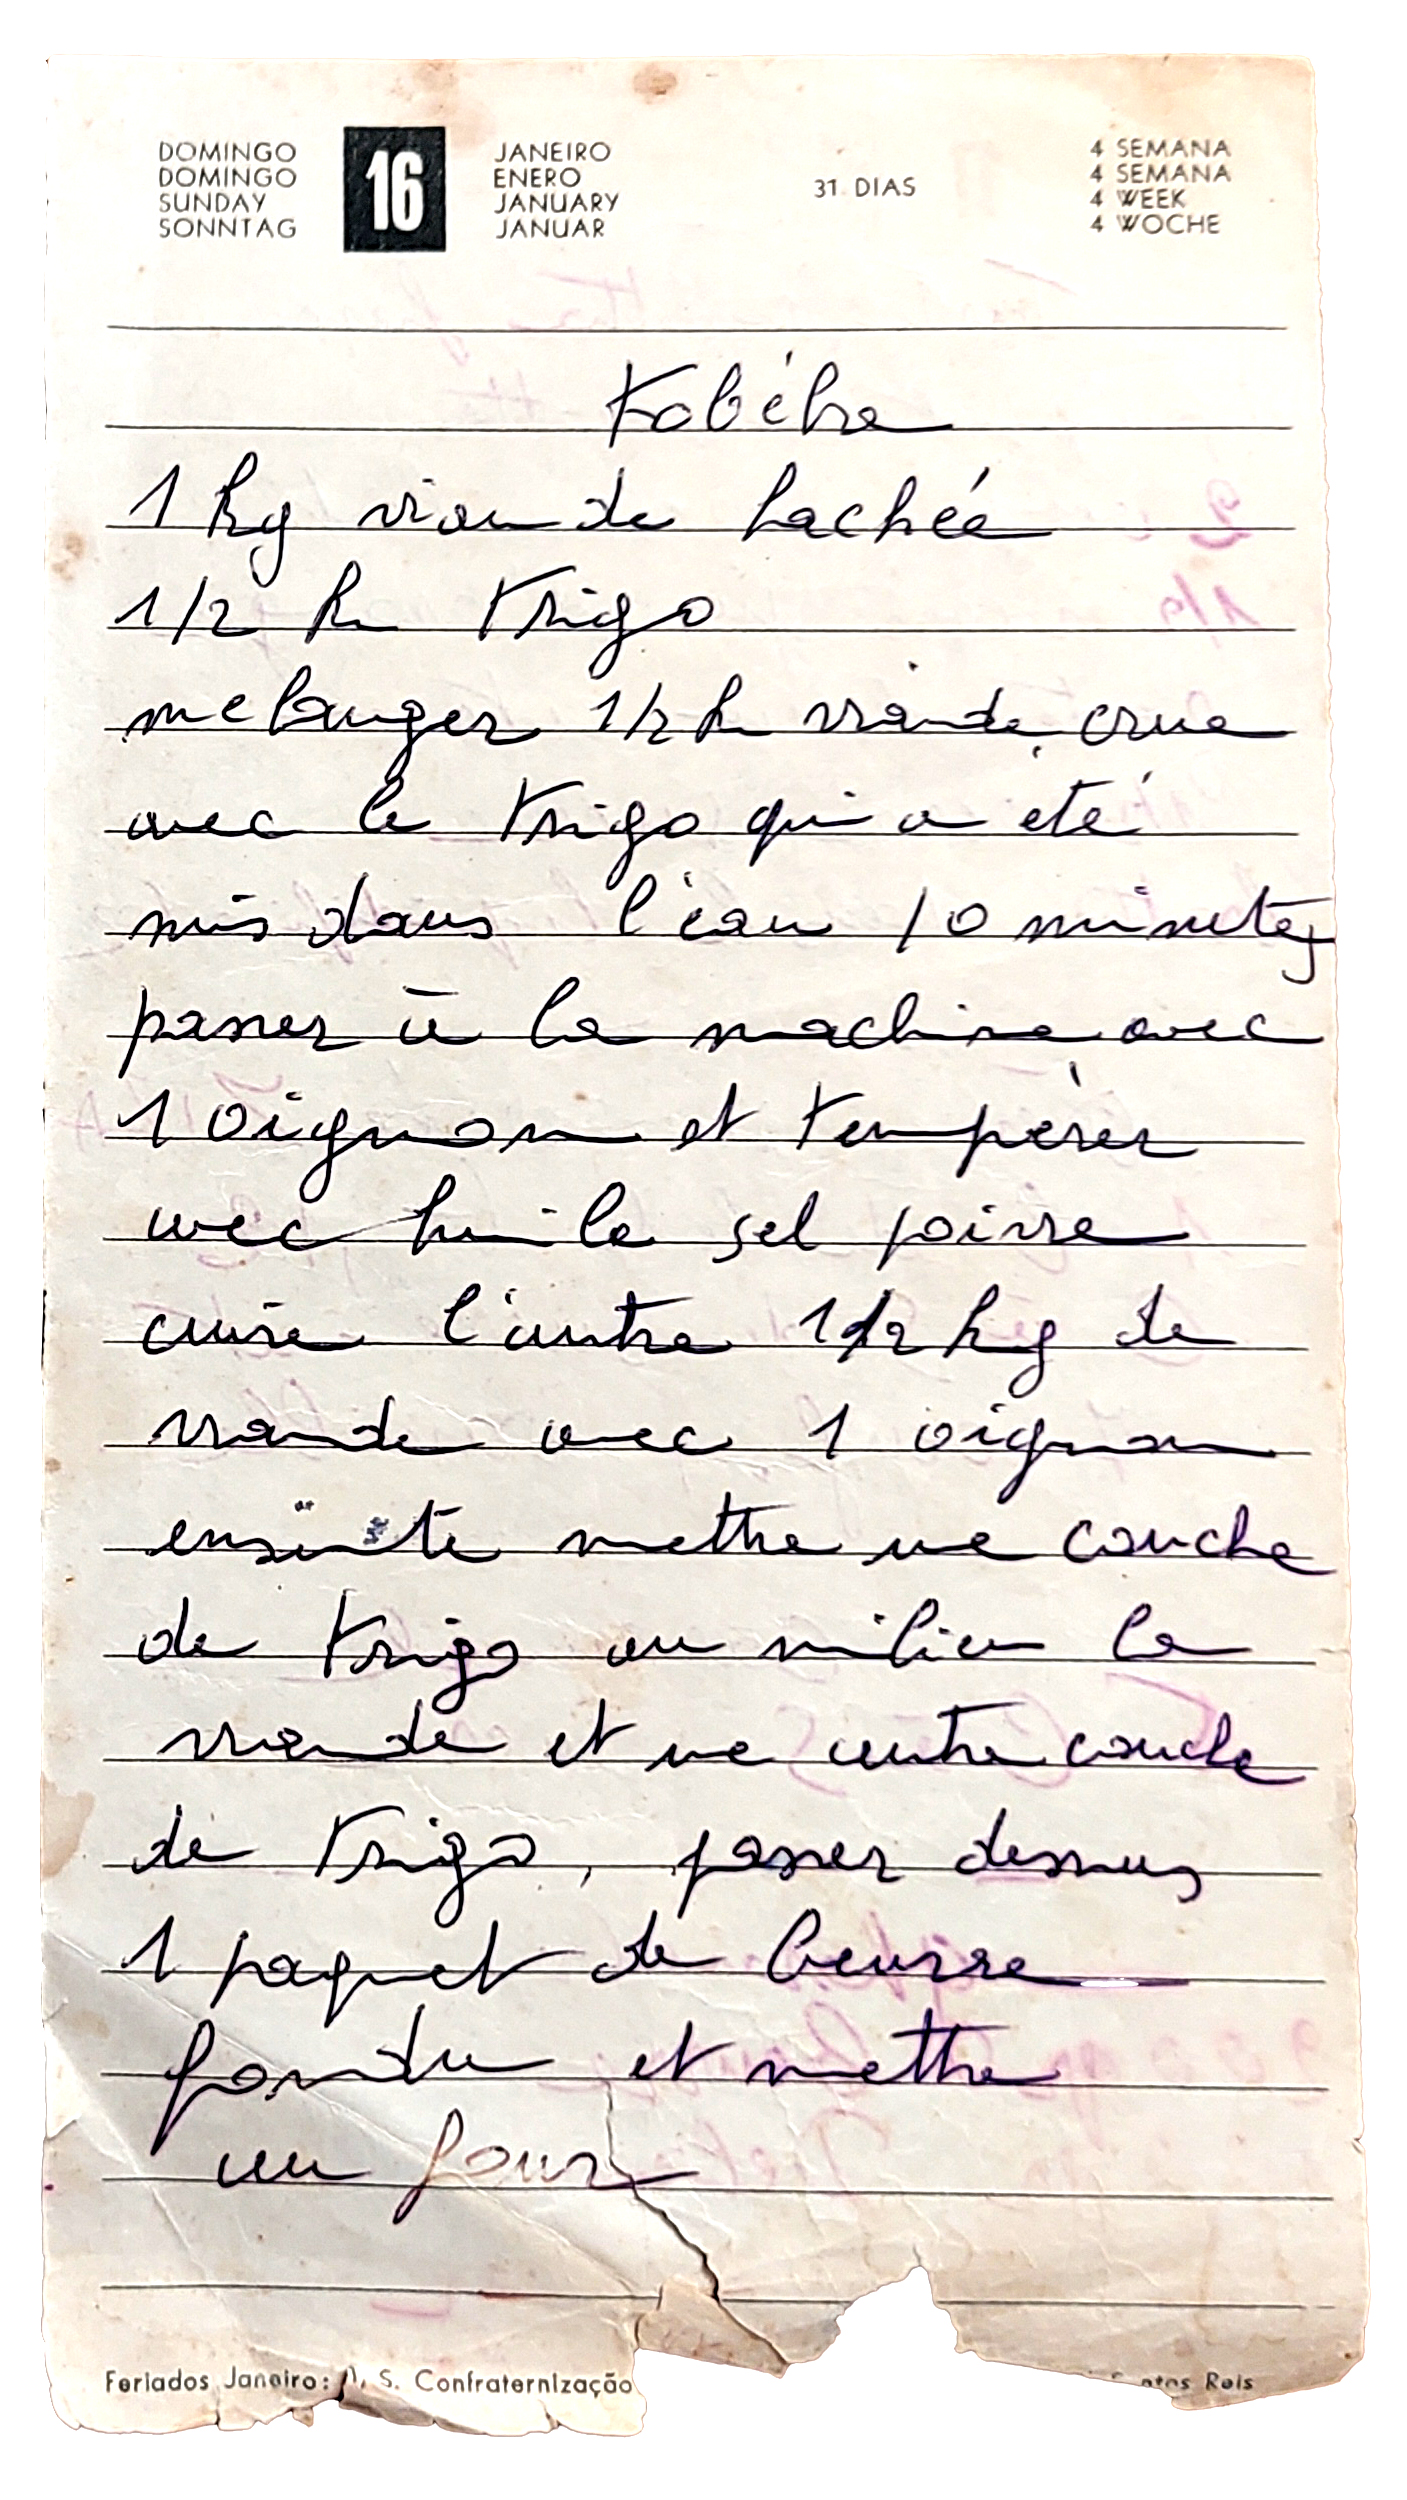
\includegraphics[width=8cm]{./recettes/edités/Kobéba.jpg}}; 
\end{tikzpicture}\clearpage\thispagestyle{empty}
% \begin{tikzpicture}[remember picture,overlay]
% \fill[black] (-3,3.5) rectangle (14,-21.5);
% \end{tikzpicture}
\clearpage

\chapter*{Kobéba}

\section{Ingrédients originaux}

\begin{itemize}
\item 1 kg viande hachée
\item 1/2 kg trigo
\item 2 oignons
\item Huile, sel, poivre
\item 1 paquet de beurre
\end{itemize}

\section{Préparation adaptée}

Misturez 1/2 kg de viande crue avec le boulgour préalablement trempé dans l’eau pendant 10 minutes et bien égoutté. Passez ce mélange au hachoir (ou mixez-le) avec 1 oignon et assaisonnez avec de l’huile, du sel et du poivre jusqu’à obtenir une préparation homogène. À part, faites revenir l’autre 1/2 kg de viande avec 1 oignon haché, en assaisonnant selon votre goût. Dans un moule huilé, étalez une couche de ce mélange de viande et de boulgour, ajoutez la viande cuite au centre puis recouvrez avec une seconde couche en lissant bien. Découpez en losanges ou en carrés, arrosez de beurre fondu et faites cuire au four préchauffé à 180°\,\textsc{c} pendant environ 30 à 40 minutes, jusqu’à ce que le dessus soit bien doré.

\chapter{Kobeba}

\section{Ingredientes originais}

\begin{itemize}
\item 1 kg de carne moída
\item 1/2 kg de trigo
\item 2 cebolas
\item Óleo, sal, pimenta
\item 1 tablete de manteiga
\end{itemize}

\section{Modo de preparo adaptado}

Misture 1/2 kg de carne crua com o trigo previamente hidratado em água por 10 minutos e bem escorrido. Passe essa mistura no moedor (ou processe) com 1 cebola e tempere com óleo, sal e pimenta até obter uma preparação homogênea. À parte, refogue o outro 1/2 kg de carne com 1 cebola picada, temperando a gosto. Em uma forma untada, espalhe uma camada dessa mistura de carne e trigo, adicione a carne cozida no centro e cubra com outra camada, alisando bem. Corte em losangos ou quadrados, regue com manteiga derretida e leve ao forno preaquecido a 180°\,\textsc{c} por cerca de 30 a 40 minutos, até que a superfície esteja bem dourada.
\blankpage

\thispagestyle{empty}
\clearpage
\begin{tikzpicture}[remember picture, overlay]
\node at (3,-7) {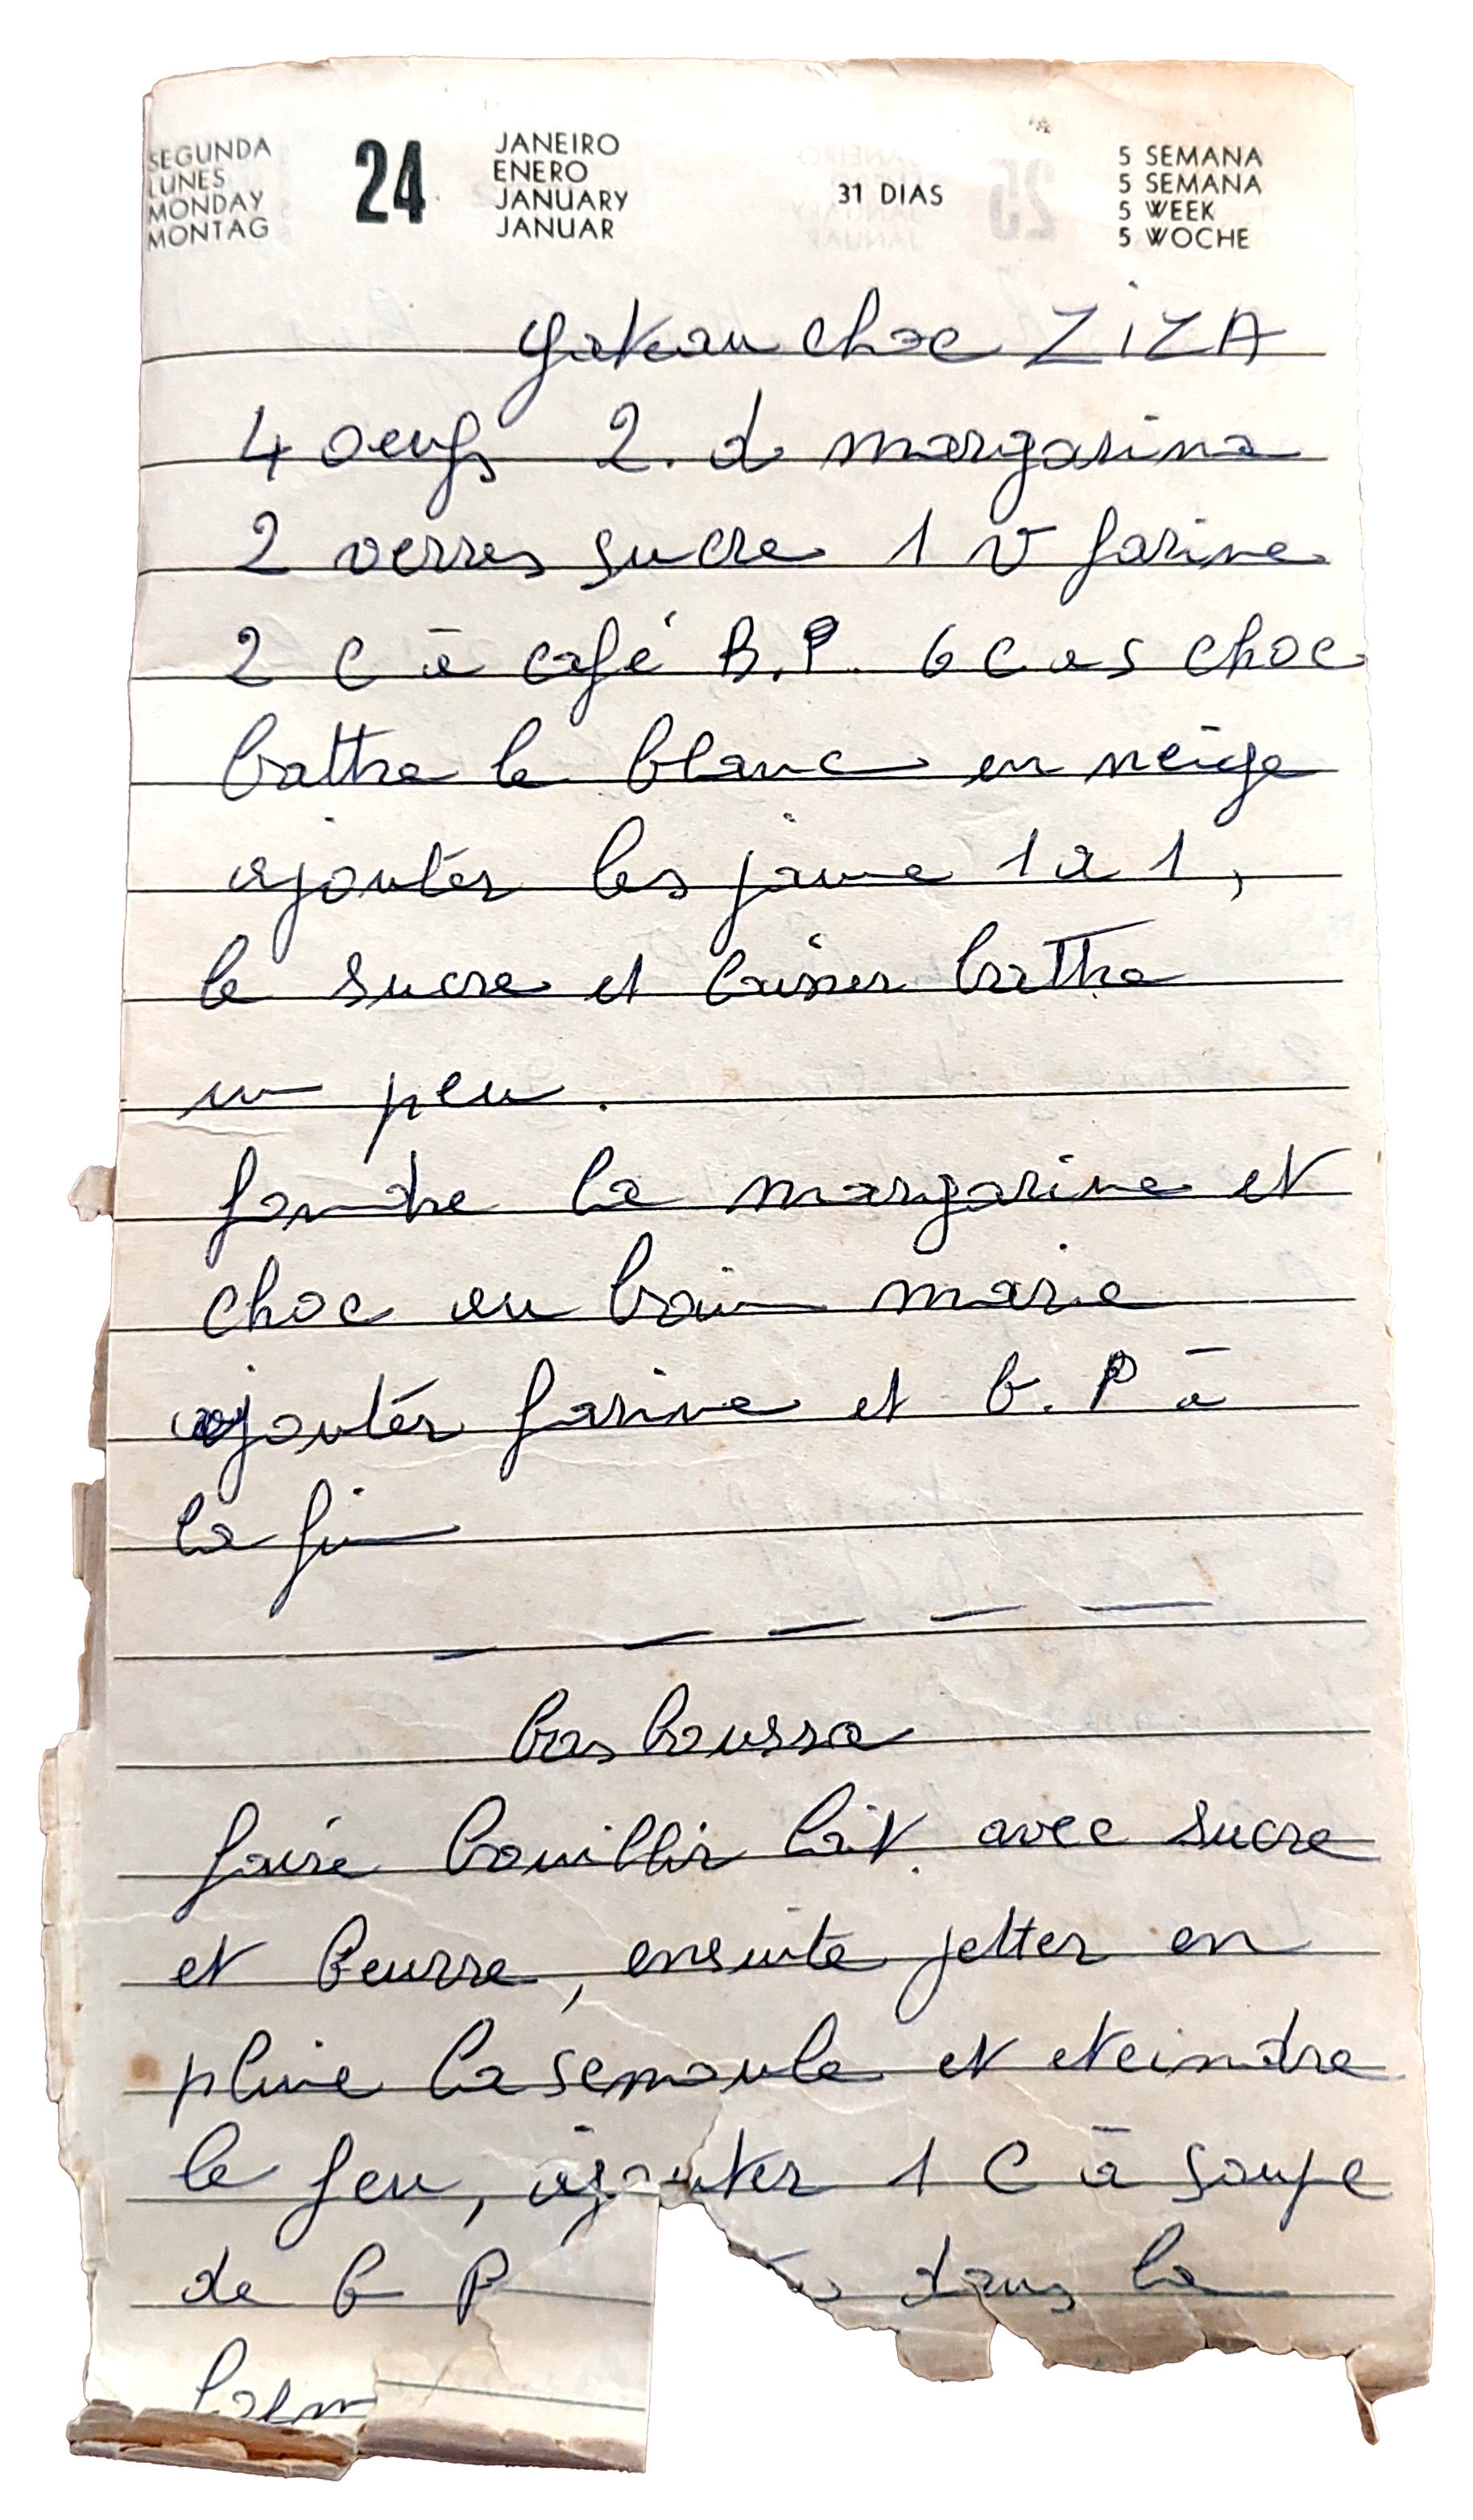
\includegraphics[width=8cm]{./recettes/edités/Gateau choc Ziza, Basboussa et Atayef (parte 1).jpg}}; 
\end{tikzpicture}\clearpage\thispagestyle{empty}
% \begin{tikzpicture}[remember picture,overlay]
% \fill[black] (-3,3.5) rectangle (14,-21.5);
% \end{tikzpicture}
\clearpage

\chapter*{Basboussa}

\section{Ingrédients originaux}

\begin{itemize}
\item Lait, sucre et beurre
\item Semoule
\item 1 c à soupe de \textsc{b.p.}
\item Pour le sirop:
	\begin{itemize}
	\item 3 verres de sucre
	\item 2 verres d’eau
	\item 1/2 citron
	\item 1 c à soupe vinaigre
	\end{itemize}
\end{itemize}

\section{Préparation adaptée}

Faites bouillir le lait avec le sucre et le beurre, versez la semoule en pluie en remuant puis retirez du feu ; laissez tiédir, ajoutez la levure chimique et mélangez. Versez dans un moule beurré et faites cuire à 180°\,\textsc{c} pendant 30--40 minutes, jusqu’à ce que le dessus soit doré ; préparez le sirop en faisant bouillir le sucre, l’eau et le citron (le vinaigre est facultatif) et, à la sortie du four, arrosez le gâteau encore chaud en laissant absorber avant de servir.

\chapter{Bolo de semolina}

\section{Ingredientes originais}

\begin{itemize}
\item Leite, açúcar e manteiga
\item Sêmola
\item 1 colher de sopa de fermento químico
\item Para a calda:
	\begin{itemize}
	\item 3 copos de açúcar
	\item 2 copos de água
	\item 1/2 limão
	\item 1 colher de sopa de vinagre
	\end{itemize}
\end{itemize}

\section{Modo de preparo adaptado}

Ferva o leite com o açúcar e a manteiga, despeje a sêmola em chuva mexendo e retire do fogo; deixe amornar, adicione o fermento químico e misture. Coloque em forma untada e asse a 180°\,\textsc{c} por 30--40 minutos, até dourar; prepare a calda fervendo açúcar, água e limão (vinagre opcional) e, ao retirar do forno, regue o bolo ainda quente, deixando absorver antes de servir.
\blankpage

\thispagestyle{empty}
\clearpage
\begin{tikzpicture}[remember picture, overlay]
\node at (3,-7) {\includegraphics[width=8cm]{./recettes/edités/Pain d'Espagne et sablé chocolat.jpg}}; 
\end{tikzpicture}\clearpage\thispagestyle{empty}
% \begin{tikzpicture}[remember picture,overlay]
% \fill[black] (-3,3.5) rectangle (14,-21.5);
% \end{tikzpicture}
\clearpage

\chapter*{Sablé au chocolat}

\section{Ingrédients originaux}

\begin{itemize}
\item 1/4 beurre
\item 2 c à s sucre
\item 2 c à s chocolat
\item farine jusqu’à ce que ça prenne
\item Pour le glaçage:
	\begin{itemize}
	\item 4 c à s choc
	\item 4 c à s sucre
	\item 1 tasse à café lait
\end{itemize}
\end{itemize}

\section{Préparation adaptée}

Mélangez le beurre avec le sucre et le chocolat, puis ajoutez la farine progressivement jusqu’à obtenir une pâte ferme et homogène. Façonnez les biscuits et faites cuire au four préchauffé à 180°\,\textsc{c} pendant environ 15 à 20 minutes. Pour le glaçage, portez à ébullition le chocolat, le sucre et le lait, retirez du feu et ajoutez une noix de beurre en mélangeant jusqu’à obtenir une texture lisse. Nappez les biscuits une fois refroidis.

\chapter{Torta de chocolate}

\section{Ingredientes originais}

\begin{itemize}
\item 1/4 de manteiga
\item 2 colheres de sopa de açúcar
\item 2 colheres de sopa de chocolate
\item farinha até dar ponto
\item Para a cobertura:
	\begin{itemize}
	\item 4 colheres de sopa de chocolate
	\item 4 colheres de sopa de açúcar
	\item 1 xícara de café de leite
\end{itemize}
\end{itemize}

\section{Modo de preparo adaptado}

Misture a manteiga com o açúcar e o chocolate, depois adicione a farinha aos poucos até obter uma massa firme e homogênea. Modele os biscoitos e leve ao forno preaquecido a 180°\,\textsc{c} por cerca de 15 a 20 minutos. Para a cobertura, leve ao fogo o chocolate, o açúcar e o leite até ferver, retire do fogo e adicione um pequeno pedaço de manteiga, misturando até obter uma textura lisa. Cubra os biscoitos depois de frios.
\blankpage

\thispagestyle{empty}
\clearpage
\begin{tikzpicture}[remember picture, overlay]
\node at (3,-7) {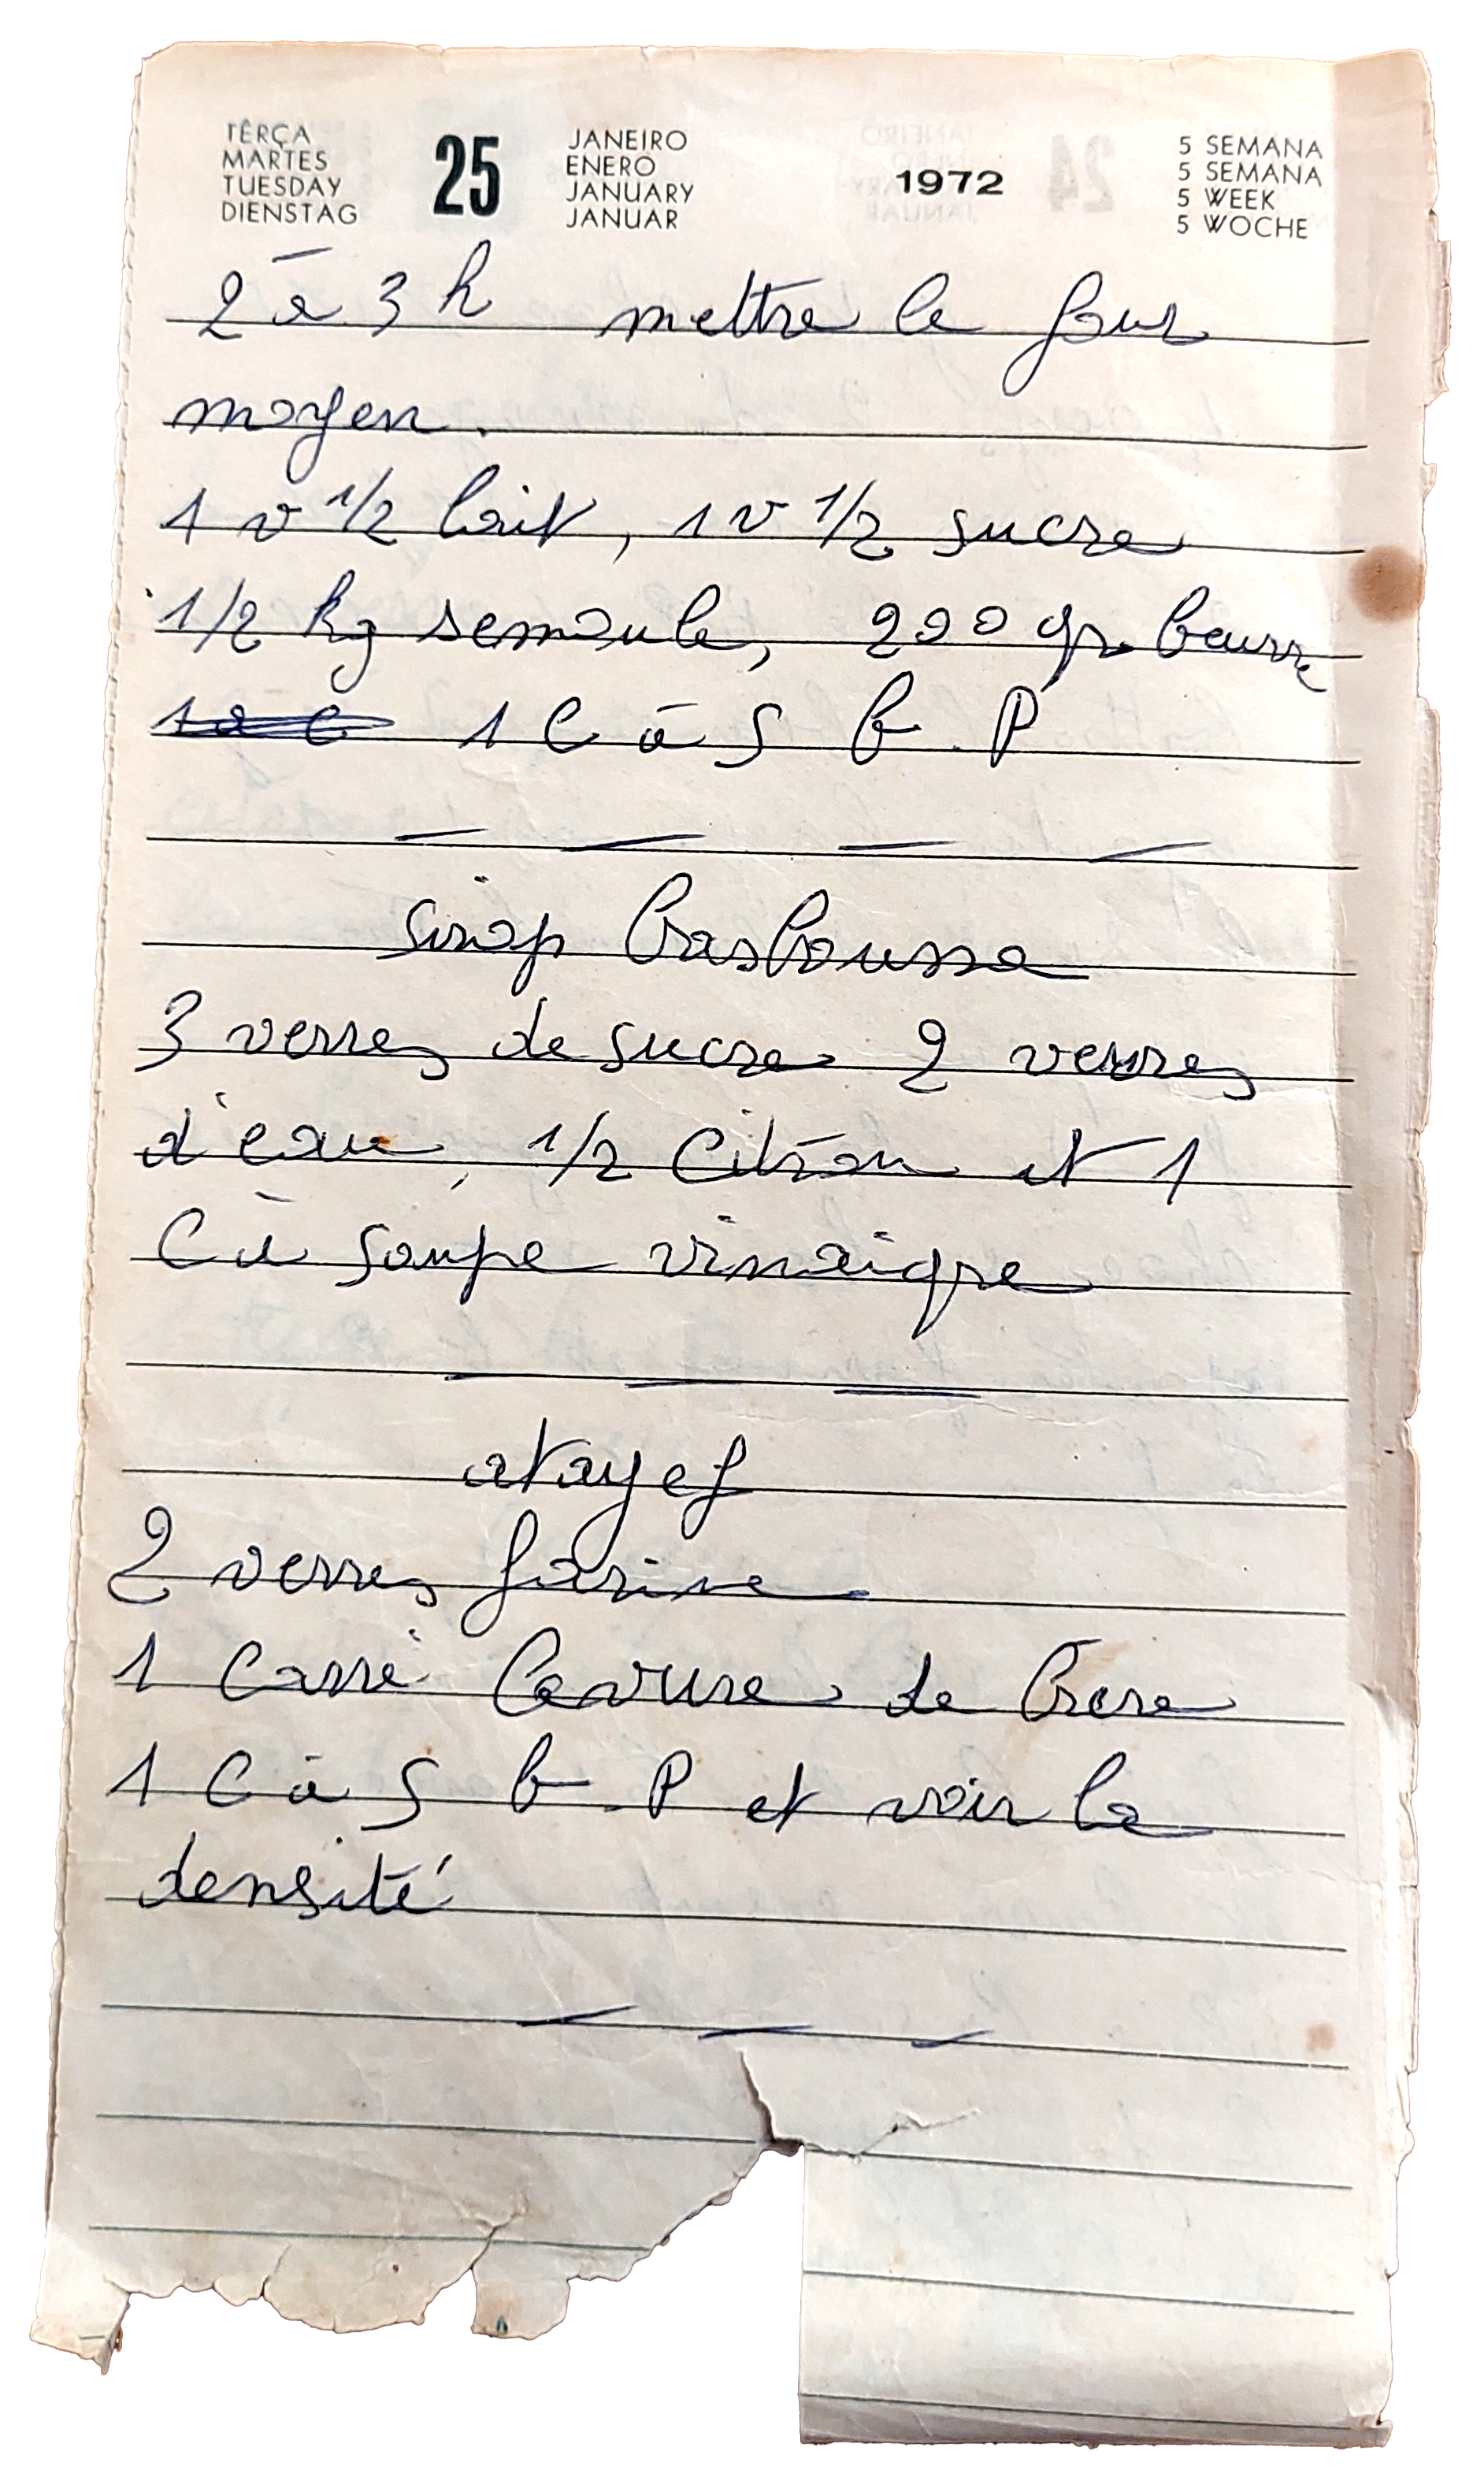
\includegraphics[width=8cm]{./recettes/edités/Gateau choc Ziza, Basboussa et Atayef (parte 2).jpg}}; 
\end{tikzpicture}\clearpage\thispagestyle{empty}
% \begin{tikzpicture}[remember picture,overlay]
% \fill[black] (-3,3.5) rectangle (14,-21.5);
% \end{tikzpicture}
\clearpage

\chapter*{Atayef}

\section{Ingrédients originaux}

\begin{itemize}
\item 2 verres farine
\item 1 case levure de bière
\item 1 c à s B.P et voir la densité
\end{itemize}

\section{Préparation adaptée}

Mélangez la farine avec la levure de boulanger et la levure chimique (\textsc{b.,p.}), puis ajoutez de l’eau tiède jusqu’à obtenir une pâte lisse, semi-liquide. Laissez reposer 30--60 minutes jusqu’à formation de bulles. Versez de petites portions dans une poêle chaude sans matière grasse et faites cuire d’un seul côté jusqu’à ce que la surface soit trouée et sèche. Laissez refroidir, puis garnissez de noix hachées mélangées avec du sucre et un peu d’eau de fleur d’oranger, et repliez en demi-lune.

\chapter{Atayef}

\section{Ingredientes originais}

\begin{itemize}
\item 2 copos de farinha
\item 1 tablete de fermento biológico
\item 1 colher de sopa de B.P. e ver a densidade
\end{itemize}

\section{Modo de preparo adaptado}

Misture a farinha com o fermento biológico e o fermento químico (\textsc{b.,p.}), depois adicione água morna até obter uma massa lisa e semilíquida. Deixe descansar por 30--60 minutos, até formar bolhas. Despeje pequenas porções em uma frigideira quente sem untar e cozinhe de um só lado, até que a superfície esteja cheia de furinhos e seca. Deixe esfriar, depois recheie com nozes picadas misturadas com açúcar e um pouco de água de flor de laranjeira, e feche em meia-lua.
%\input{Y-publicidade}	   % [lista de livros publicados]
\input{Z-colofon}		   % [colofon]